\section{Desarrollo}

Inicialmente, como el problema así planteado es difícil de abordar, se simplificó de las siguientes maneras:

\begin{itemize}
	\item La trayectoria rectilínea que se busca será paralela al eje $Y$ y simétrica respecto del plano $XZ$ del robot.
	\item Se desarrollará para X positivos.
\end{itemize}

Estas simplificaciones permiten desarrollar las consignas sin perder valor educativo y además permite hacer una demostración en vivo. La Figura \ref{fig:trayectorias verticales} ilustra las trayectorias propuestas.


\begin{figure}[H]
	\centering
	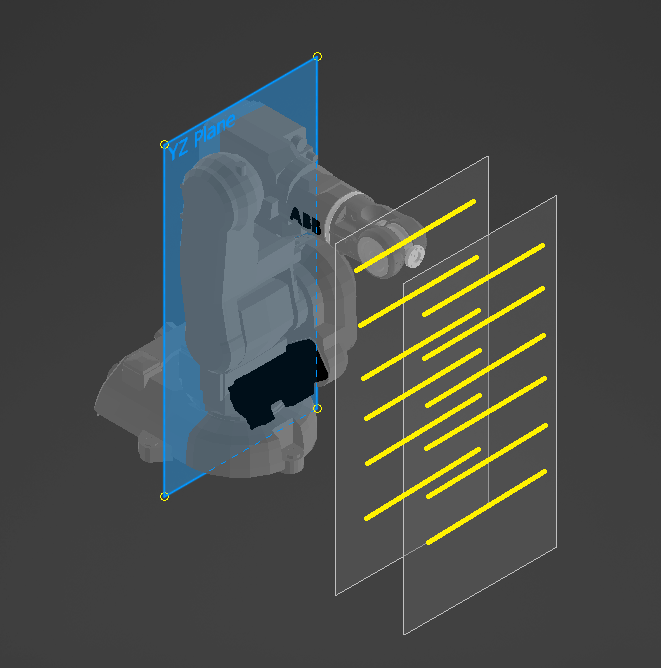
\includegraphics[width=0.5\textwidth]{./img/trayectorias.png}
	\caption{Trayectorias horizontales a evaluar}
	\label{fig:trayectorias verticales}
\end{figure}


\subsection{Teoría}

El jacobiano es función de las variables articulares, y relaciona las velocidades articulares con la velocidades cartesianas. Para una pose dada, el jacobiano indica, entre otras cosas, la capacidad de desarrollar velocidad del robot en esa pose. Una trayectoria se puede pensar como una secuencia de poses, cada una con su propio jacobiano.

\begin{equation}
\begin{bmatrix}
	v \\
	\omega
\end{bmatrix}
=
J(q)\cdot \dot{q}
\end{equation}

Si el robot ha de moverse en una trayectoria cartesiana lineal a velocidad constante, la velocidad máxima posible será la menor velocidad que se dé entre 2 poses consecutivas de la trayectoria. Es decir, el robot se moverá tan rápido como permita el segmento de la trayectoria más lento. En términos matemáticos, si definimos $\mathcal{V}$ como el conjunto de velocidades que se desarrollan en una trayectoria, la velocidad constante máxima será el valor mínimo del set.

\begin{equation}
	\mathcal{V} = \{ v_0, v_1, \dots, v_{N-1} \}
\end{equation}

\begin{equation}
	v_{cte}^{\max} =\min \mathcal{V} = \min_{i \in \{0,\dots,N-1\}} v_i
\end{equation}

Suponiendo que el robot puede desarrollar sus velocidades articulares máximas, es posible calcular la velocidad cartesiana máxima teórica para cada punto de una trayectoria. Luego, la velocidad constante máxima en la dirección del movimiento será la velocidad cartesiana mínima encontrada proyectada sobre dicha dirección.

Esto último parece bien conceptualmente, pero no se ajusta a la realidad, porque no tiene en cuenta que, si el robot se mueve a velocidad angular máxima siempre, la trayectoria que la herramienta desarrolle no va a ser lineal.

Otra forma de encarar el problema es evaluar la trayectoria desde un enfoque cinemático diferencial (de a pedacitos), imponiendo directamente la condición de movimiento cartesiano rectilíneo y analizando las exigencias articulares que esto implica. En este sentido, para cada punto del recorrido se calcula, a partir de la inversa de la matriz Jacobiana, la velocidad angular que debe desarrollar cada articulación para sostener el avance en la dirección deseada a velocidad unitaria.

\begin{equation}
	\dot{\mathbf{q}} = \mathbf{J}(\mathbf{q})^{-1} \mathbf{v}
\end{equation}

\begin{equation}
	\dot{\mathbf{q}}_{req} = | \mathbf{J}(\mathbf{q})^{-1} \mathbf{\hat{v}} |
\end{equation}

 Estas velocidades requeridas se comparan con los límites máximos de cada actuador, identificando en cada instante cuál de ellos actúa como cuello de botella y, por lo tanto, fija la velocidad cartesiana máxima admisible en ese punto. Finalmente, dado que la consigna exige mantener velocidad constante a lo largo de toda la trayectoria, se adopta como velocidad de ejecución el valor más restrictivo entre todos los puntos evaluados, garantizando así que el movimiento completo pueda realizarse sin saturar ningún motor.

\begin{equation}
	v_{p} = \min_{i} \left( \frac{\dot{q}_{max,i}}{\dot{q}_{req,i}} \right)
\end{equation}


Con todo esto dicho, es posible crear un programa que calcule una solución numérica con un algoritmo de \textit{brute-force} que evalúe las trayectorias del tipo $(X_0,-100,Z_0) \to (X_0,100,Z_0)$ para todo el plano de trabajo $X$,$Z$  del robot.



\section{Metodología para la Optimización de la Trayectoria}

Para determinar la ubicación óptima que permita ejecutar una trayectoria rectilínea de 200\,mm en el menor tiempo posible (a velocidad constante), se implementó un método de barrido espacial (\textit{Grid Search}). Esta estrategia evalúa conceptualmente el espacio de trabajo del manipulador basándose en los siguientes principios:

\subsection{Exploración del Espacio de Trabajo}
Se define una cuadrícula de evaluación sobre el plano $YZ$ que abarca el volumen de alcance físico útil del robot. En cada coordenada de esta cuadrícula, se proyecta la trayectoria rectilínea deseada. Esto se realiza para distintos planos paralelos al YZ a diferentes distancias.

\subsection{Análisis Cinemático Diferencial}
Cada trayectoria propuesta se evalúa punto por punto a lo largo de su recorrido. Utilizando la matriz Jacobiana del robot, se relacionan los límites físicos de velocidad de cada motor con la velocidad cartesiana resultante en la herramienta. Esto permite identificar qué articulación se satura primero en cada instante, dictando la velocidad máxima posible en ese punto específico.

\subsection{Restricción de Velocidad Constante}
Dado que la consigna exige que la velocidad se mantenga constante durante los 200\,mm, la velocidad máxima admisible para una trayectoria entera queda estrictamente limitada por su ``punto más lento'' (el cuello de botella cinemático a lo largo de esa recta). El algoritmo registra y compara estas velocidades mínimas sostenibles para encontrar la ubicación global más rápida.


\section{Resultados y análisis}
El algoritmo fue llevado a cabo para trayectorias horizontales para distintos planos paralelos al YZ como se indico en las secciones anteriores. La Figura \ref{fig:mapa_horizontal} presenta un mapa de calor de la velocidad máxima para cada trayectoria evaluada. A partir de los resultados del algoritmo, se observa que, para este tipo de trayectoria, la velocidad máxima alcanzable es de \SI{2,7}{m/s}, y se obtiene en la posición (\SI{775}{mm}, \SI{131}{mm}).

\begin{figure}[H]
		\centering
		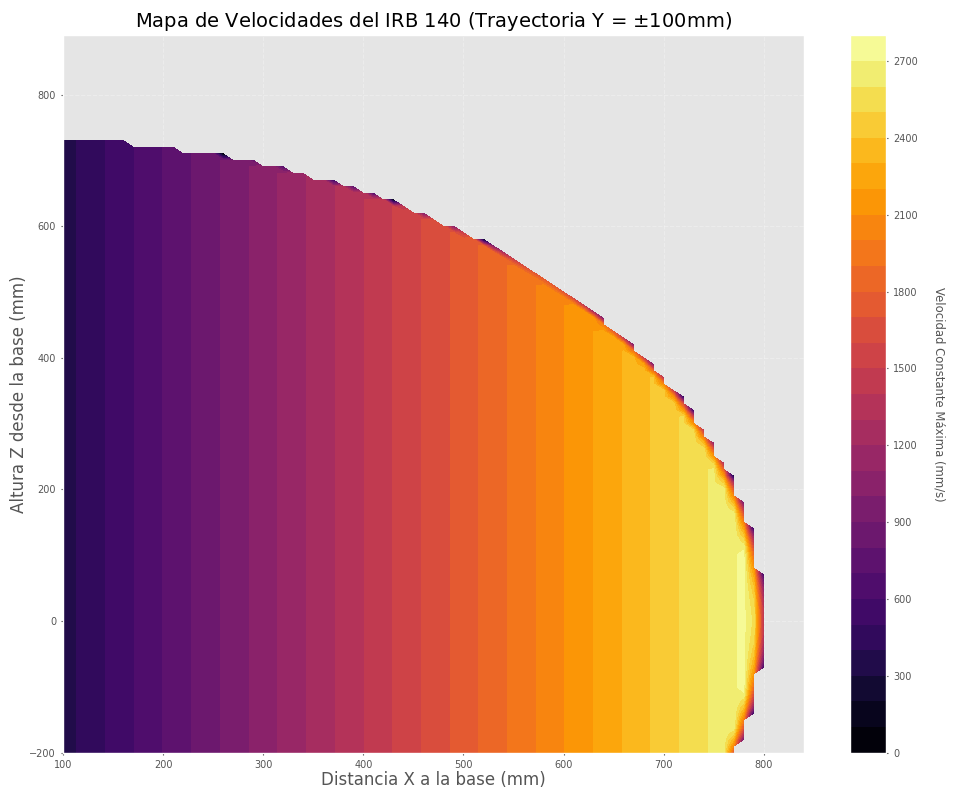
\includegraphics[width=0.7\textwidth]{./img/mapa_calor_xz.png}
		\caption{Mapa de calor de velocidades máximas para trayectorias horizontales}
		\label{fig:mapa_horizontal}
\end{figure}

A fin de evaluar otras posibles trayectorias el algoritmo fue ejecutado pero para trayectorias verticales contenidas en el plano YZ. Similarmente, la Figura \ref{fig:mapa_vertical} muestra el mapa de calor obtenido. La velocidad máxima alcanzable es de \SI{2,25}{m/s}, y se obtiene en la posición (\SI{675}{mm}, \SI{-125}{mm}).

\begin{figure}[h]
	\centering
	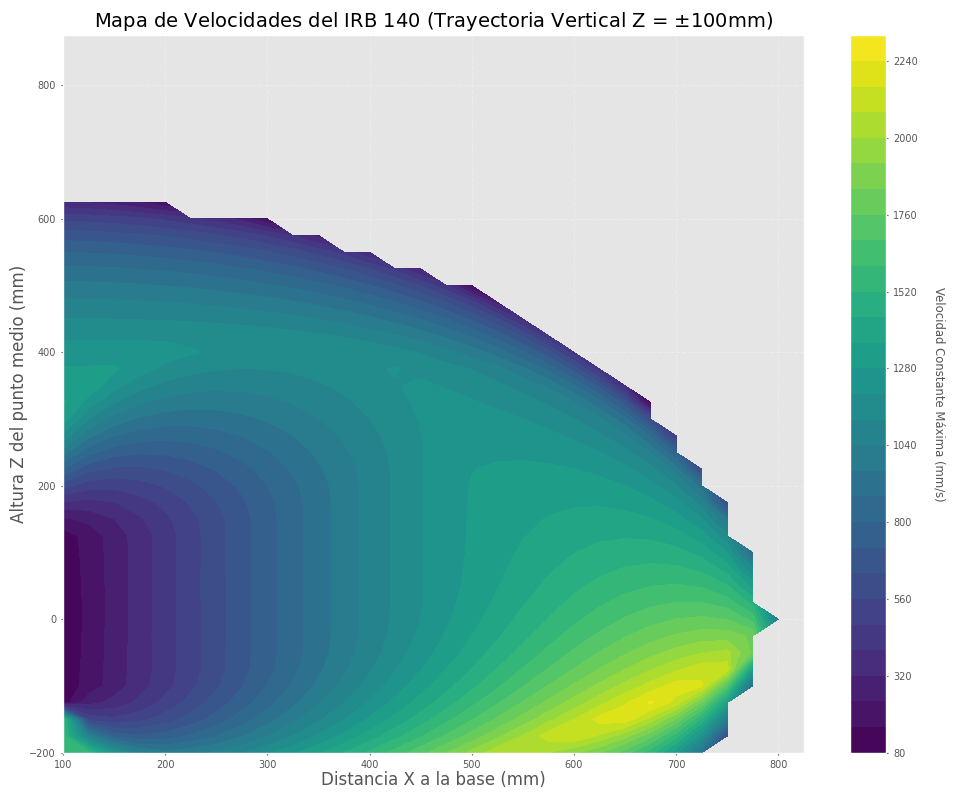
\includegraphics[width=0.7\textwidth]{./img/mapa_calor_verticales.png}
	\caption{Mapa de calor de velocidades máximas para trayectorias verticales}
	\label{fig:mapa_vertical}
\end{figure}


En el caso de trayectorias horizontales, el mapa de calor muestra que las trayectorias que pueden recorrerse en menor tiempo se concentran cuando el brazo del robot se encuentra casi completamente extendido y a alturas cercanas a la base. Este comportamiento resulta consistente, ya que la velocidad lineal aumenta con la distancia al eje de rotación. En consecuencia, los movimientos asociados al eje 1 generan un incremento significativo en la velocidad del extremo del brazo.

Respecto de las trayectorias verticales, el comportamiento no resulta tan evidente. Los menores tiempos se obtienen cuando el brazo se encuentra considerablemente extendido y con una inclinación pronunciada hacia adelante. Asimismo, se observa que las velocidades alcanzadas son significativamente menores que en las trayectorias horizontales. Esto puede explicarse por el hecho de que este tipo de movimiento no requiere rotaciones del eje 1, por lo que no contribuye de manera significativa a la velocidad lineal.

\clearpage

La figura \ref{fig:y-vs-t-y-velocidad} muestra los resultados de la simulación realizada en \textit{RoboStudio}. El programa se mueve con un movimiento tipo \textit{joint} desde un punto alejado de la trayectoria hasta su inicio, luego hace un movimiento lineal sin limite de velocidad, y termina la secuencia volviendo al origen previamente mencionado; la secuencia se repite 2 veces. Se usó ``$z=$\textit{fine}'' para que la simulación respete el inicio y fin de la trayectoria. Se aclara que se eligió una terna de \textit{tool0} con un eje Z apuntando ``hacia abajo'' ya que no se supo como configurarla solidaria a la terna 3, que sería la más adecuada para como se resolvió el problema.

La velocidad presenta un pico en la trayectoria lineal, que es razonable ya que el robot intenta moverse lo más rápido posible, pero su aceleración es finita. En términos físicos, es imposible lograr que la trayectoria se resuelva a velocidad constante si no se le da espacio para tomar carrera antes\footnote{Esto se probó pero no es posible para una trayectoria tan cerca del limite de la esfera de alcance del robot.}.

La velocidad promedio medida es de \SI{487.1735}{\mm\per\s}, muy lejos de los \SI{2,7}{\m \per \s} calculados numéricamente. Dicho esto, la discrepancia es fácilmente explicable por 2 cosas:
\begin{enumerate}
	\item La simulación numérica realizada no contempla las mismas limitaciones que \textit{RoboStudio}.
	\item El robot no tomó carrera antes; si se hace esto la velocidad aumenta drásticamente.
\end{enumerate}

En sí, el resultado es considerado adecuado y válido, para las limitaciones impuestas por nosotros mismos y la física del robot.

\begin{figure}[h!]
	\centering
	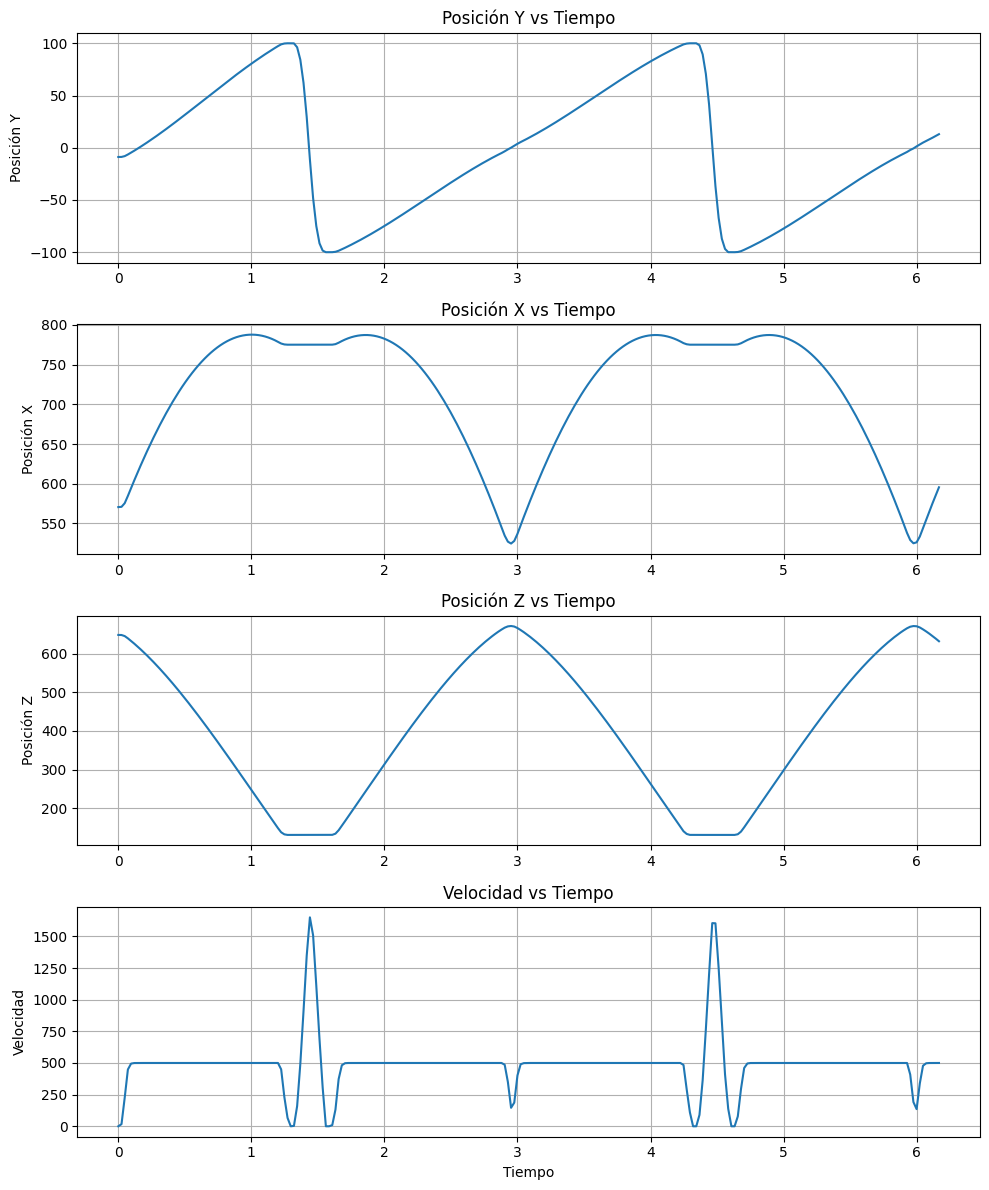
\includegraphics[width=0.7\linewidth]{img/Y vs t y velocidad}
	\caption{Posición y velocidad en función del tiempo}
	\label{fig:y-vs-t-y-velocidad}
\end{figure}


Ahora bien, para el caso de la trayectoria vertical, la simulación devolvió los datos de la imagen \ref{}. Se usaron las mismas configuraciones que antes.





